\documentclass[12pt]{article}

\usepackage[margin=0.5in]{geometry}
\usepackage{amsmath, amssymb}
\usepackage{hyperref}
\usepackage{tikz}
\renewcommand{\arraystretch}{1.6}

% Header pset untuk halaman pertama
\newcommand{\psetheader}[4]{%
  \noindent
  \begin{minipage}[t]{0.6\textwidth}
    #1\\
    #2\\
    #3
  \end{minipage}%
  \hfill
  \begin{minipage}[t]{0.35\textwidth}
    \raggedleft #4
  \end{minipage}

  \vspace{0.5\baselineskip}
  \hrule
  \vspace{1em}
}

\title{Matematika Dasar - Tugas 2}
\author{Anas Azhar \ FST - Matematika - 056413438 \ Universitas Terbuka}
\date{\today}

\begin{document}

\psetheader
  {\textit{Matematika Dasar} - Tugas 2}
  {Universitas Terbuka, FST - Matematika, 2025.1}
  {Anas Azhar (056413438)}
  {Minggu, 9 November 2025}

\section*{Soal 1}
\textbf{Diketahui:}
\[
A = \{3,4\}, \qquad B = \{2,4,5,6\}.
\]

\noindent Buatlah relasi dalam bentuk pasangan terurut sesuai syarat berikut:
\[
R_1 = \{(a,b)\mid a \ge b,\; a \in A,\; b \in B\},
\qquad
R_2 = \{(a,b)\mid a + 1 \ge b,\; a \in A,\; b \in B\}.
\]

\section*{Penyelesaian}

\subsection*{a. Relasi \(R_1\)}

Uji setiap pasangan \((a,b)\) dengan syarat \(a \ge b\):

\[
\begin{aligned}
a = 3 &: (3,2)\ \text{memenuhi}, \\
a = 4 &: (4,2),\ (4,4)\ \text{memenuhi}.
\end{aligned}
\]

Maka:
\[
\boxed{
R_1 = \{(3,2),\ (4,2),\ (4,4)\}
}
\]

\subsection*{b. Relasi \(R_2\)}

Uji setiap pasangan \((a,b)\) dengan syarat \(a + 1 \ge b\):

\[
\begin{aligned}
a = 3 &: (3,2),\ (3,4)\ \text{memenuhi}, \\
a = 4 &: (4,2),\ (4,4),\ (4,5)\ \text{memenuhi}.
\end{aligned}
\]

Sehingga diperoleh:
\[
\boxed{
R_2 = \{(3,2),\ (3,4),\ (4,2),\ (4,4),\ (4,5)\}
}
\]

\section*{Soal 2}
Diketahui himpunan bilangan bulat
\[
\mathbb{Z} = \{\ldots,-2,-1,0,1,2,\ldots\}
\]
dan relasi
\[
aRb \iff b = 3a,\quad a\in\mathbb{Z},\; b\in\mathbb{Z}.
\]

\textbf{Domain} relasi $R$ didefinisikan sebagai
\[
D(R) = \{a \in \mathbb{Z} \mid \exists\, b \in \mathbb{Z} \text{ sehingga } aRb\}.
\]
Karena untuk setiap $a \in \mathbb{Z}$ selalu dapat dipilih $b = 3a \in \mathbb{Z}$,
maka
\[
D(R) = \mathbb{Z}.
\]

\textbf{Range} relasi $R$ didefinisikan sebagai
\[
R(R) = \{b \in \mathbb{Z} \mid \exists\, a \in \mathbb{Z} \text{ sehingga } aRb\}.
\]
Dengan syarat $aRb \iff b = 3a$, maka semua $b$ yang mungkin adalah kelipatan 3,
yaitu
\[
R(R) = \{3a \mid a \in \mathbb{Z}\} = \{\ldots,-6,-3,0,3,6,\ldots\} = 3\mathbb{Z}.
\]

Jadi:
\[
\boxed{D(R) = \mathbb{Z}, \qquad R(R) = 3\mathbb{Z}}.
\]

\section*{Soal 3}
\textbf{Diketahui graf berikut:}

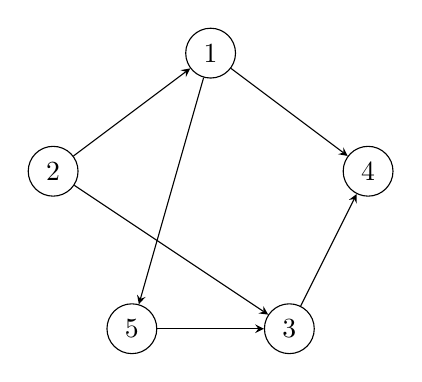
\begin{tikzpicture}[>=stealth, node distance=2cm]
    % gaya simpul
    \tikzstyle{vertex}=[circle,draw,minimum size=18pt,inner sep=0pt]

    % posisi simpul
    \node[vertex] (1) at (0,2) {1};
    \node[vertex] (2) at (-2,0.5) {2};
    \node[vertex] (4) at (2,0.5) {4};
    \node[vertex] (5) at (-1,-1.5) {5};
    \node[vertex] (3) at (1,-1.5) {3};

    % panah (relasi)
    \draw[->] (2) -- (1);      % 2 -> 1
    \draw[->] (2) -- (3);      % 2 -> 3
    \draw[->] (1) -- (4);      % 1 -> 4
    \draw[->] (1) -- (5);      % 1 -> 5
    \draw[->] (5) -- (3);      % 5 -> 3
    \draw[->] (3) -- (4);      % 3 -> 4
\end{tikzpicture}

\noindent \textbf{Soal:}
\begin{enumerate}
    \item[a.] Buatlah relasi dalam bentuk pasangan terurut dari graf di atas.
    \item[b.] Periksa apakah relasi tersebut bersifat refleksif, simetris, dan transitif.
\end{enumerate}

\section*{Penyelesaian}

Dari graf tampak panah:
\[
2 \to 1,\quad
2 \to 3,\quad
1 \to 4,\quad
1 \to 5,\quad
5 \to 3,\quad
3 \to 4.
\]

Maka himpunan titik:
\[
A = \{1,2,3,4,5\}.
\]

\subsection*{a. Relasi dalam bentuk pasangan terurut}

Setiap panah $a \to b$ membentuk pasangan $(a,b)$. Maka relasi:
\[
R = \{(2,1),\ (2,3),\ (1,4),\ (1,5),\ (5,3),\ (3,4)\}.
\]

\subsection*{b. Pemeriksaan sifat relasi}

\textbf{1. Refleksif}

Relasi dikatakan refleksif jika $(x,x) \in R$ untuk semua $x \in A$.

Pada graf tidak ada loop, sehingga
\[
(1,1),\ (2,2),\ (3,3),\ (4,4),\ (5,5) \notin R.
\]
Maka:
\[
R \text{ tidak refleksif.}
\]

\textbf{2. Simetris}

Relasi simetris jika $(a,b)\in R$ mengakibatkan $(b,a)\in R$.

Karena
\[
(2,1)\in R \quad \text{tetapi} \quad (1,2)\notin R,
\]
maka:
\[
R \text{ tidak simetris.}
\]

\textbf{3. Transitif}

Relasi transitif jika $(a,b)\in R$ dan $(b,c)\in R$ mengakibatkan $(a,c)\in R$.

Perhatikan:
\[
(2,1)\in R \quad \text{dan} \quad (1,4)\in R,
\]
tetapi
\[
(2,4)\notin R.
\]
Sehingga:
\[
R \text{ tidak transitif.}
\]

\section*{Kesimpulan}
\[
\boxed{
R \text{ tidak refleksif, tidak simetris, dan tidak transitif.}
}
\]

\end{document}